
\chapter{Appendix}

\section{Control System Logic Diagram}
Figure 4 represents the saw state behaviour in a logic flow diagram.
\begin{figure}
		\centering
		\includegraphics[width=8in,angle=90]{../DRAWINGS/wo19011.pdf}
		\caption{Saw Control Logic}
		\label{fig:Saw-Logic}
\end{figure}
\pagebreak
\section{Control System Wiring Diagrams}
The following drawings are the electrical drawings for the Saw Control System. They are included in the manual for quick reference.
\paragraph*{Wiring Diagrams}for the Saw Control System.
\begin{center}
	\includegraphics[width=7.5in,angle=90]{../DRAWINGS/19011-000.pdf}
	\captionof{figure}{}\label{schem:cover} % optional
\end{center}
\begin{center}
	\includegraphics[width=7.5in,angle=90]{../DRAWINGS/19011-001.pdf}
	\captionof{figure}{Drawing Listing}\label{schem:toc} % optional
\end{center}
\begin{center}
	\includegraphics[width=7.5in,angle=90]{../DRAWINGS/19011-002.pdf}
	\captionof{figure}{Main Power Connections}\label{schem:002} % optional
\end{center}
\begin{center}
	\includegraphics[width=7.5in,angle=90]{../DRAWINGS/19011-003.pdf}
	\captionof{figure}{Emergency Stop, DC Power, PLC Power, MCR Circuit}\label{schem:003} % optional
\end{center}
\begin{center}
	\includegraphics[width=7.5in,angle=90]{../DRAWINGS/19011-004.pdf}
	\captionof{figure}{Safety Gate Interlock Connections}\label{schem:004} % optional
\end{center}
\begin{center}
	\includegraphics[width=7.5in,angle=90]{../DRAWINGS/19011-005.pdf}
	\captionof{figure}{Saw Motor and Soft Starter Connections}\label{schem:005} % optional
\end{center}
\begin{center}
	\includegraphics[width=7.5in,angle=90]{../DRAWINGS/19011-006.pdf}
	\captionof{figure}{Control Communication Network, Long Axis Sensors}\label{schem:006} % optional
\end{center}
\begin{center}
	\includegraphics[width=7.5in,angle=90]{../DRAWINGS/19011-007.pdf}
	\captionof{figure}{Vertical and Cross axii Drives and Motors Connections}\label{schem:007} % optional
\end{center}
\begin{center}
	\includegraphics[width=7.5in,angle=90]{../DRAWINGS/19011-008.pdf}
	\captionof{figure}{Long Travel Drives and Motors Connections}\label{schem:008} % optional
\end{center}
\begin{center}
	\includegraphics[width=7.5in,angle=90]{../DRAWINGS/19011-009.pdf}
	\captionof{figure}{PLC Input Wiring}\label{schem:009} % optional
\end{center}
\begin{center}
	\includegraphics[width=7.5in,angle=90]{../DRAWINGS/19011-010.pdf}
	\captionof{figure}{PLC Output Wiring}\label{schem:010} % optional
\end{center}
\begin{center}
	\includegraphics[width=7.5in,angle=90]{../DRAWINGS/19011-011.pdf}
	\captionof{figure}{Analog Input and Output Wiring}\label{schem:011} % optional
\end{center}
\section{AV20 Encoder}
\begin{center}
	\includegraphics[width=5.5in]{afiles/FX1.pdf}
	\label{av20:1} % optional
\end{center}
\begin{center}
	\includegraphics[width=6.0in]{afiles/FX2.pdf}
	\label{av20:2} % optional
\end{center}
\begin{center}
	\includegraphics[width=6.0in]{afiles/FX3.pdf}
	\label{av20:3} % optional
\end{center}
\begin{center}
	\includegraphics[width=6.0in]{afiles/FX4.pdf}
	\label{av20:4} % optional
\end{center}
\section{Dynapar Potential Encoder Replacements}
\begin{center}
	\includegraphics[width=5.5in]{afiles/E23_DS_701949_2.pdf}
	\label{e23} % optional
\end{center}
\section{Schneider Electric Potential Encoder Replacements}
\begin{center}
	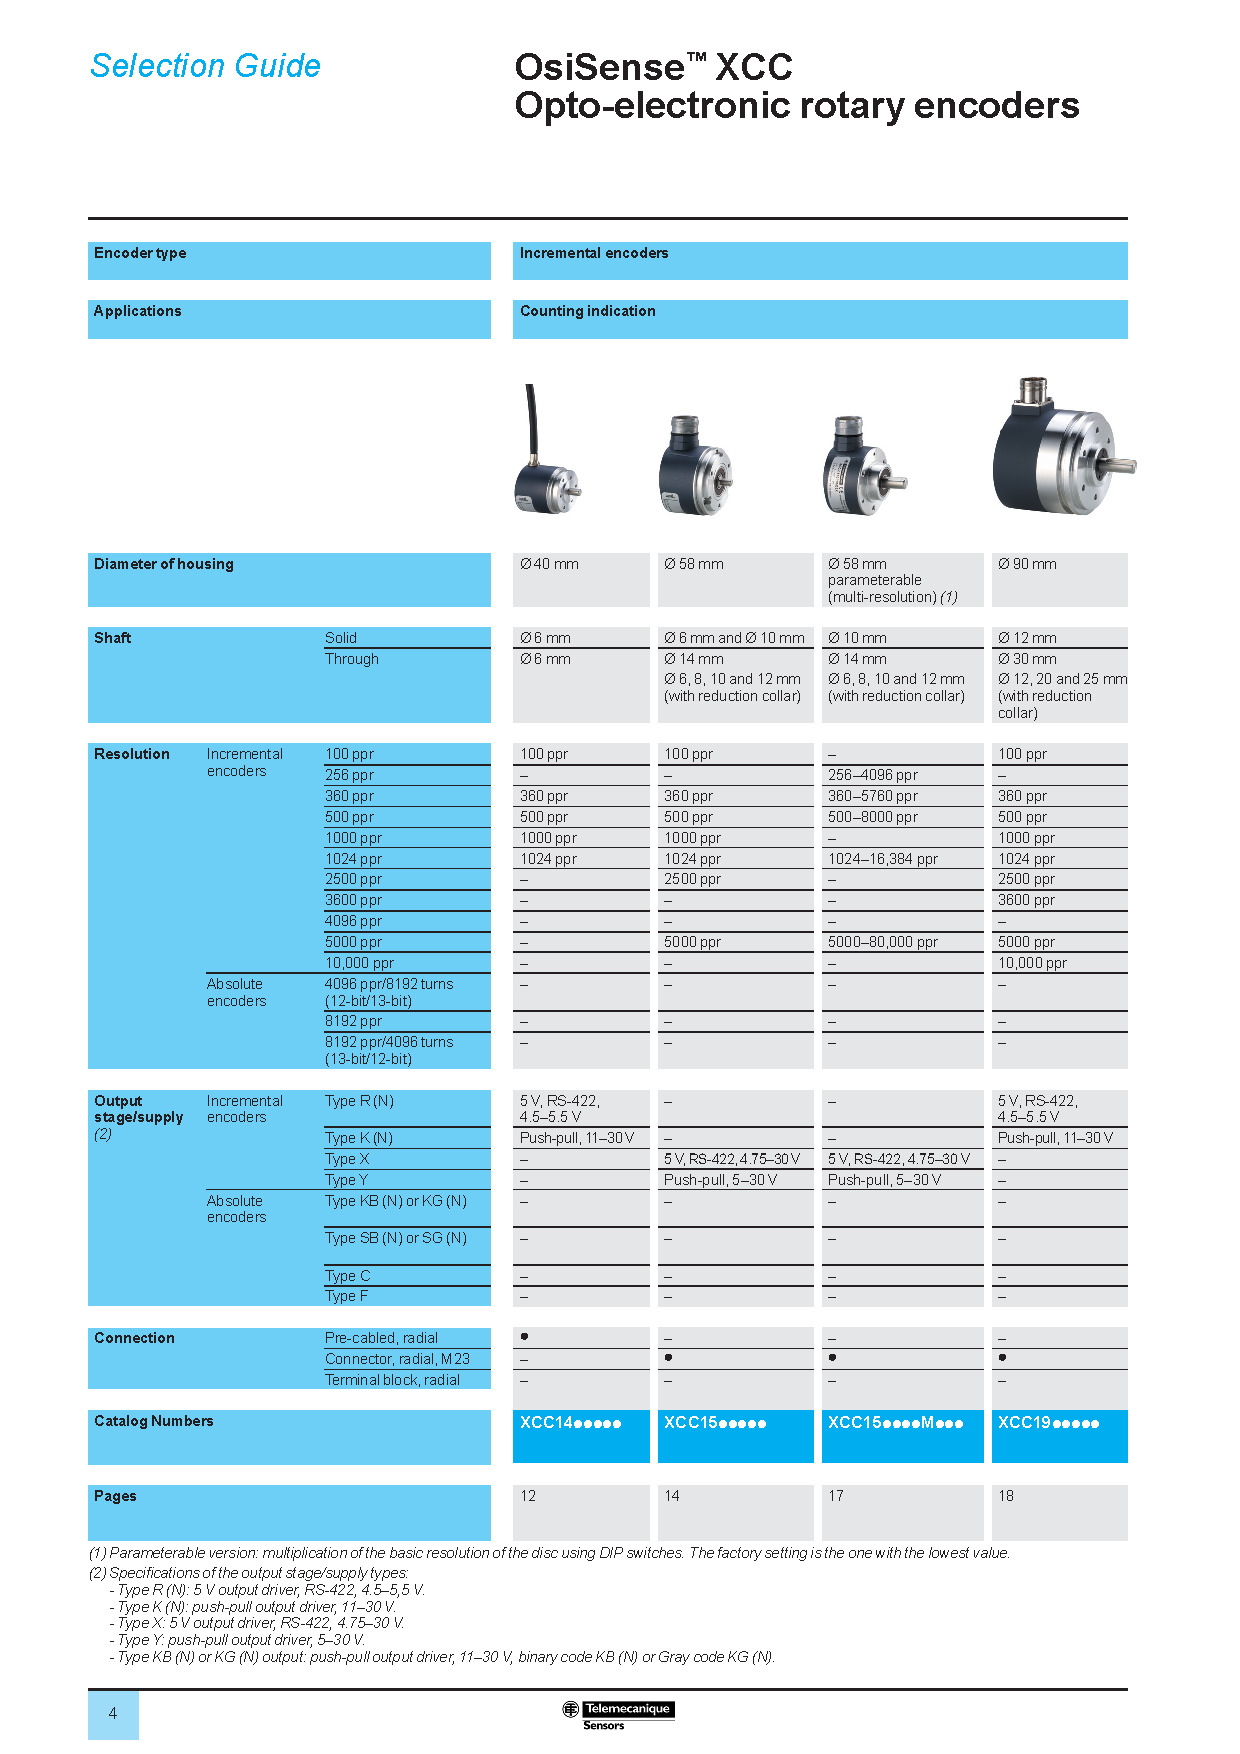
\includegraphics[width=5.5in]{afiles/9006CT1101 Encoders.pdf}
	\label{xcc} % optional
\end{center}
\section{Original Manual Pages}
\begin{center}
	\includegraphics[width=5.5in]{afiles/manold1.pdf}
	\label{om1} % optional
\end{center}
\begin{center}
	\includegraphics[width=6.0in]{afiles/manold2.pdf}
	\label{om2} % optional
\end{center}
\begin{center}
	\includegraphics[width=6.0in]{afiles/manold3.pdf}
	\label{om3} % optional
\end{center}
\begin{center}
	\includegraphics[width=6.0in]{afiles/manold4.pdf}
	\label{om4} % optional
\end{center}
\begin{center}
	\includegraphics[width=6.0in]{afiles/manold5.pdf}
	\label{om5} % optional
\end{center}
\begin{center}
	\includegraphics[width=6.0in]{afiles/manold6.pdf}
	\label{om6} % optional
\end{center}
\begin{center}
	\includegraphics[width=6.0in]{afiles/manold7.pdf}
	\label{om7} % optional
\end{center}
\begin{center}
	\includegraphics[width=6.0in]{afiles/manold8.pdf}
	\label{om8} % optional
\end{center}